\documentclass{article}
\usepackage{amsmath}
\usepackage{graphicx}
\graphicspath{ {./images/} }
\usepackage{hyperref}
\usepackage[nameinlink,capitalize]{cleveref}
\usepackage[dvipsnames]{xcolor}

\definecolor{green}{RGB}{0, 152, 112}
\definecolor{orange}{RGB}{230, 160, 0}
\definecolor{ligthblue}{RGB}{154, 208, 243}
\definecolor{darkblue}{RGB}{0, 116, 180}
\definecolor{orangered}{RGB}{213, 94, 0}
\definecolor{lavender}{RGB}{203, 121, 167}
\definecolor{yellow}{RGB}{240, 228, 66}

\addtolength{\oddsidemargin}{-.875in}
\addtolength{\evensidemargin}{-.875in}
\addtolength{\textwidth}{1.75in}
\addtolength{\topmargin}{-.875in}
\addtolength{\textheight}{1.75in}

\title{\normalfont{Back propagation in a simple neural net}}
\author{HappyDustbunny}

\begin{document}
\maketitle
\section*{Introduction}
Brains are made up of neurons connected to each other. By making a mathematical model of some neurons wired together (a neural network) one can emulate some aspects of a brain.
\\
In this note we will look at a very simple neural network in detail and show how matrices can be used to describe the processing and learning of the network.
\\The matrix formulation works for bigger networks as well.
\\
The goal of this note is to look at a simple example in painstaking detail. For more background and analysis go to the links in the references at the end of the note. \cite{Mazur}
\\
\\
\section*{The basic model}
The network we will consider here consists of two input neurons (or nodes), two output neurones and a single hidden layer with two neurons.
\\
That simple a network can only transform two input numbers, say (0.1, 0.9), to two output numbers, say (0.3, 0.4).
\\
In the Open Office Calc document \textit{Simple\_Neural\_Net.ods} such a network is implementet in a spreadsheet.
\\
\\
The layers are numbered with the input layer as (0), the hidden layer as (1) and the output layer as (2). \textit{In this note an upper index in parenthesis refer to the layer.}
\\
In each layer there are two neurons numbered 0 and 1 with \textit{a lower index}.
\\
Every neuron has a value $a$ with indices indicating which neuron it belongs to.
\\
For example $a_0^{(0)}$ is the value of the first (input) neuron in the first layer.
\begin{figure}[h]
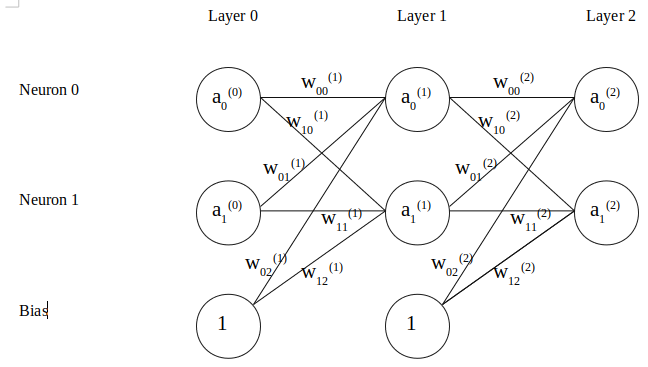
\includegraphics[scale=.4]{two_neuron_net}
\centering
\end{figure}
\\
Each neuron in a layer is connected to every neuron in the previous layer (except the Input layer of course).\\
\\
The weights between two layers "belongs" to the layer with the higher number and to make use of matrices easier the indices of each weight $w$ is has the number of the end-neuron written before the number of the input neuron.
\\
Therefore $w_{01}^{(1)}$ is the weight between the neurons with values $a_1^{(0)}$ and $a_0^{(1)}$.
\\
A bias is added to each weighted sum in order to avoid origo (Origo: the starting point of the coordinate system. "(0, 0)") always being a minimum.
\\
\\
Instead of keeping tabs of the biases separately we will use a bias node for each layer with a value of 1 and store the actual biases as the weights for this node. This helps keep the matrix formulation simple.
\\
Here $w_{02}^{(1)}$ and $w_{12}^{(1)}$ is the biases for layer (1).
\\
\\
The value of a neuron is a function of the weighted sum of the neuron values from previous layers. $$a_0^{(1)} = f(\sum_{i=0}^{1}{w_{0i}^{(1)}a_i^{(0)}}+w_{12}^{(1)})$$
\\
The function introduces a needed non-linearity and keeps the numbers manageable.
\\
A lot of functions can be used, but a common choice is the sigmoid function $\sigma(x) = \dfrac{1}{(1-e^{-x})} = \dfrac{e^{x}}{(1-e^{x})}$ with the practical derivative $\sigma(x) = \sigma(x)(1 - \sigma(x)) $.
\\
\\
\begin{figure}[h]
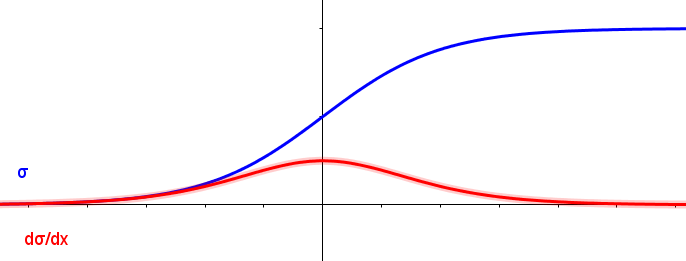
\includegraphics[scale=.5]{sigmoid}
\centering
\end{figure}
\\
To train the network input values are fed into the input nodes, the weighted sum is calculated for the hidden layer and then for the output layer. This is called \textit{the forward pass}.
\\
Then the output values are compared to target values $T_0, T_1, ...$ and a \textit{cost} is calculated. This cost is a function of all the weights and using the derivative of the cost function with respect to each weight an adjustment to the weights can be \textit{back propagated}.
\\
\section*{Forward pass}
In the forward pass the values of each neuron is calculated by applying the sigmoid function to the weighted sum of input for each layer:
\\
\begin{equation} \label{eq:a01}
a_0^{(1)} = \sigma(w_{00}^{(1)}a_0^{(0)}+w_{01}^{(1)}a_1^{(0)}+w_{02}^{(1)})
\end{equation}
\begin{equation} \label{eq:a11}
a_1^{(1)} = \sigma(w_{10}^{(1)}a_0^{(0)}+w_{11}^{(1)}a_1^{(0)}+w_{12}^{(1)})
\end{equation}
\\
\begin{equation} \label{eq:a02}
a_0^{(2)} = \sigma(w_{00}^{(2)}a_0^{(1)}+w_{01}^{(2)}a_1^{(1)}+w_{02}^{(2)})
\end{equation}
\begin{equation} \label{eq:a12}
a_1^{(2)} = \sigma(w_{10}^{(2)}a_0^{(1)}+w_{11}^{(2)}a_1^{(1)}+w_{12}^{(2)})
\end{equation}
Or in matrix notation:
\[
\vec a^{(1)} =
\binom{a_0^{(1)}}{a_1^{(1)}} =
\sigma \left ( \binom{w_{00}^{(1)}a_0^{(0)}+w_{01}^{(1)}a_1^{(0)}+w_{02}^{(1)}}{w_{10}^{(1)}a_0^{(0)}+w_{11}^{(1)}a_1^{(0)}+w_{12}^{(1)}} \right )
= \sigma\left((a_0^{(0)} a_1^{(0)} 1)
\begin{pmatrix}
w_{00}^{(1)} & w_{10}^{(1)} \\
w_{01}^{(1)} & w_{11}^{(1)} \\
 w_{02}^{(1)} & w_{12}^{(1)}
\end{pmatrix}\right)
= \sigma(\vec A^{(0)}W^{(1)})
\]
In the same way
\[
\vec a^{(2)} = \sigma(\vec A^{(1)}W^{(2)})
\]
Note that $\vec a^{(1)} = \binom{a_0^{(1)}}{a_1^{(1)}}$ and $\vec A^{(1)} = (a_0^{(1)} a_1^{(1)} 1)$ both contain the values for the nodes in layer (1).
\\
$\vec A^{(1)}$ is needed to include the biases in some calculations.
\\
\section*{Back propagation}
To train the network we need a measure of how far the output values $\vec a^{(2)}$ are from the target values $\vec T$. As mentioned before this measure is called \textit{the cost function}.
\\
We define the cost as the difference between output values and target values. To avoid negative numbers we square the difference before we sum up the differnces.
\\
And as the cost is just a number we want to minimize, we can multiply with $\frac{1}{2}$ to simplify the derivative.
\\
\\
In this case the cost function will be $$ C = \frac {1}{2}(a_0^{(2)}-T_0)^2 + \frac {1}{2}(a_1^{(2)}-T_1)^2 $$
or using \eqref{eq:a02} and \eqref{eq:a12}

\begin{equation} \label{eq:C}
\begin{aligned}
C = \frac {1}{2}(\sigma(w_{00}^{(2)}a_0^{(1)}+w_{01}^{(2)}a_1^{(1)}+w_{02}^{(2)})-T_0)^2 +
\\
\frac {1}{2}(\sigma(w_{10}^{(2)}a_0^{(1)}+w_{11}^{(2)}a_1^{(1)}+w_{12}^{(2)})-T_1)^2
\end{aligned}
\end{equation}
\\
To minimize the cost we find the derivative of C with respect to each weight in layer (2).
\\
This derivative can be subtracted from the relevant weights in order to get a better cost value after the next forward pass.
\\
Note that the derivative of \textit{all} weights in \textit{all} layers have to be calculated before \textit{any} weight is changed.
\\
\\
Let's start by finding $\frac{dC}{dw_{00}^{(2)}}$
\\
Only the first term of C in equation \eqref{eq:C} include $w_{00}^{(2)}$.
\\
This term is a composite function $f \circ g \circ h(w_{00}^{(2)}, w_{01}^{(2)}, w_{02}^{(2)}, w_{10}^{(2)}, w_{11}^{(2)},w_{12}^{(2)})$ where $f, g$ and $h$ and their derivatives are
$$f(\sigma) = \frac {1}{2}(\sigma-T_0)^2~~~~~~~~~~~~~~~~~~~~~~~~~~~~~~~~~~~~~~~~~\frac{df}{d\sigma} = \textcolor{darkblue}{(\sigma-T_0)}$$
$$g(h) = \sigma(h)~~~~~~~~~~~~~~~~~~~~~~~~~~~~~~~~~~~~~~~~~~\frac{dg}{dh} = \frac{d\sigma}{dh} = \textcolor{green}{\sigma(h)(1 - \sigma(h))}$$
$$h(w_{00}^{(2)}, w_{01}^{(2)}, w_{02}^{(2)}) = w_{00}^{(2)}a_0^{(1)}+w_{01}^{(2)}a_1^{(1)}+w_{02}^{(2)}~~~~~~~~\frac{dh}{dw_{00}^{(2)}} = \textcolor{orange}{a_0^{(1)}}$$
By using  \eqref{eq:a02} we note that $$(\sigma - T_0) = \textcolor{darkblue}{(a_0^{(2)} - T_0)}$$ and $$\sigma(h)(1-\sigma(h)) = \textcolor{green}{a_0^{(2)}(1-a_0^{(2)})}$$
\\
The chain rule $$\frac{dC}{dw_{00}^{(2)}} = \frac{df}{d\sigma}~\frac{d\sigma}{dh}~\frac{dh}{dw_{00}^{(2)}}$$
then gives us
$\frac{dC}{dw_{00}^{(2)}} = \textcolor{darkblue}{(a_0^{(2)}-T_0)}~\textcolor{green}{a_0^{(2)}(1-a_0^{(2)})}~\textcolor{orange}{a_0^{(1)}} $, the first entry in the change matrix.
\\
\\
The rest is found in a similar manner:
$$\begin{pmatrix}
\frac{dC}{dw_{00}^{(2)}} & \frac{dC}{dw_{01}^{(2)}} & \frac{dC}{dw_{02}^{(2)}}
\\\\
\frac{dC}{dw_{10}^{(2)}} & \frac{dC}{dw_{11}^{(2)}} & \frac{dC}{dw_{12}^{(2)}}
\end{pmatrix} =
$$
$$\begin{pmatrix}
\textcolor{darkblue}{(a_0^{(2)}-T_0)a_0^{(2)}(1-a_0^{(2)})}a_0^{(1)} & \textcolor{darkblue}{(a_0^{(2)}-T_0)a_0^{(2)}(1-a_0^{(2)})}a_1^{(1)} & \textcolor{darkblue}{(a_0^{(2)}-T_0)a_0^{(2)}(1-a_0^{(2)})}1
\\\\
\textcolor{green}{(a_1^{(2)}-T_1)a_1^{(2)}(1-a_1^{(2)})}a_0^{(1)} & \textcolor{green}{(a_1^{(2)}-T_1)a_1^{(2)}(1-a_1^{(2)})}a_1^{(1)} & \textcolor{green}{(a_1^{(2)}-T_1)a_1^{(2)}(1-a_1^{(2)})}1
\end{pmatrix}$$
We note that each entry in the upper row contains $\delta_0^{(2)} = \textcolor{darkblue}{(a_0^{(2)}-T_0)a_0^{(2)}(1-a_0^{(2)})}$ and that each entry in the lower row contains $\delta_1^{(2)} = \textcolor{green}{(a_1^{(2)}-T_1)a_1^{(2)}(1-a_1^{(2)})}$.
\\
\\
Therefore the \textit{transposed} change matrix for layer (2) is $$\frac{dC}{dW^{(2)}} =
\begin{pmatrix}
\frac{dC}{dw_{00}^{(2)}} & \frac{dC}{dw_{01}^{(2)}} & \frac{dC}{dw_{02}^{(2)}}
\\\\
\frac{dC}{dw_{10}^{(2)}} & \frac{dC}{dw_{11}^{(2)}} & \frac{dC}{dw_{12}^{(2)}}
\end{pmatrix} = \begin{pmatrix}
\delta_0^{(2)}a_0^{(1)} & \delta_0^{(2)}a_1^{(1)} & \delta_0^{(2)} \cdot 1
\\\\
\delta_1^{(2)}a_0^{(1)} & \delta_1^{(2)}a_1^{(1)} & \delta_1^{(2)} \cdot 1
\end{pmatrix} = \delta^{(2)}A^{(1)}
$$
where $\delta^{(2)} = \binom{\delta_0^{(2)}}{\delta_1^{(2)}}$
and we had $A^{(1)} = (a_0^{(1)} a_1^{(1)} 1)$.
\\
After all change matrices is found the change is applied to all weights. For layer (2) this will be $$W^{(2)} = W^{(2)} - \gamma \cdot \frac{dC}{dW^{(2)}}$$
where $\gamma$ is a number between 0 and 1 called the learning rate. A good start value for $\gamma$ is usually 0.5
\\
\\
To find how much each weight in layer (1) have to change we can use \textcolor{green}{\eqref{eq:a01}} and \textcolor{darkblue}{\eqref{eq:a11}} in \eqref{eq:C}

\begin{equation} \label{eq:C1}
\begin{aligned}
C = \frac {1}{2} \left(\sigma\left(w_{00}^{(2)}\textcolor{green}{\sigma(w_{00}^{(1)}a_0^{(0)}+w_{01}^{(1)}a_1^{(0)}+w_{02}^{(1)})}
+w_{01}^{(2)}\textcolor{darkblue}{\sigma(w_{10}^{(1)}a_0^{(0)}+w_{11}^{(1)}a_1^{(0)}+w_{12}^{(1)})}+w_{02}^{(2)}\right)-T_0\right)^2 +
\\
\frac {1}{2}\left(\sigma\left(w_{10}^{(2)}\textcolor{green}{\sigma(w_{00}^{(1)}a_0^{(0)}+w_{01}^{(1)}a_0^{(0)}+w_{02}^{(1)})}+w_{11}^{(2)}\textcolor{darkblue}{\sigma(w_{10}^{(1)}a_0^{(0)}+w_{11}^{(1)}a_1^{(0)}+w_{12}^{(1)})}+w_{12}^{(2)}\right)-T_1\right)^2
\end{aligned}
\end{equation}
\\
We want to find $\frac{dC}{dw_{00}^{(1)}}$ and note that $w_{00}^{(1)}$ occur in both terms of \eqref{eq:C1}.
\\
The first term is again a composite function, just a little more complicated: $f \circ g \circ h \circ k \circ m(w_{00}^{(2)}, w_{01}^{(2)}, w_{02}^{(2)}, w_{10}^{(2)}, w_{11}^{(2)},w_{12}^{(2)})$ where $f, g$, $h$, $k$ and $m$ and their derivatives are
$$f(\sigma) = \frac {1}{2}(\sigma-T_0)^2~~~~~~~~~~~~~~~~~~~~~~~~~~~~~~~~~~~~~~~~~\textcolor{darkblue}{\frac{df}{d\sigma} = (\sigma-T_0)}$$
$$g(h) = \sigma(h)~~~~~~~~~~~~~~~~~~~~~~~~~~~~~~~~~~~~~~~~~~\frac{dg}{dh} = \textcolor{green}{\frac{d\sigma}{dh} = \sigma(h)(1 - \sigma(h))}$$
$$h(w_{00}^{(2)}, w_{01}^{(2)}, w_{02}^{(2)}) = w_{00}^{(2)}\sigma(w_{00}^{(1)...})+w_{01}^{(2)}\sigma(w_{10}^{(1)...})+w_{02}^{(2)}~~~~~~~~\textcolor{orange}{\frac{dh}{d\sigma(w_{00}^{(1)...})}} = w_{00}^{(2)}$$
$$k(m) = \sigma(m)~~~~~~~~~~~~~~~~~~~~~~~~~~~~~~~~~~~~~~~~~~\frac{dk}{dm} = \textcolor{lavender}{\frac{d\sigma}{dm} = \sigma(m)(1 - \sigma(m))}$$
$$m(w_{00}^{(1)}, w_{01}^{(1)}, w_{02}^{(1)}) = w_{00}^{(1)}a_0^{(0)}+w_{01}^{(1)}a_1^{(0)}+w_{02}^{(1)}~~~~~~~~\textcolor{orangered}{\frac{dm}{dw_{00}^{(1)}} = a_0^{(0)}}$$.
\\
Using the chain rule again
$$\frac{dC}{dw_{00}^{(1)}} = \textcolor{darkblue}{\frac{df}{d\sigma}}~\textcolor{green}{\frac{d\sigma}{dh}}~\textcolor{orange}{\frac{dh}{d\sigma}}~\textcolor{lavender}{\frac{d\sigma}{dm}}~\textcolor{orangered}{\frac{dm}{dw_{00}^{(1)}}}+\ldots$$
and remembering that $$\textcolor{green}{\sigma(h) = a_0^{(2)}} ~\textnormal{and}~ \textcolor{lavender}{\sigma(m) = a_0^{(1)}}$$
then gives us the first term in the first entry of the new change matrix:
$$\frac{dC}{dw_{00}^{(1)}} = \textcolor{darkblue}{(a_0^{(2)}-T_0)}~\textcolor{green}{a_0^{(2)}(1-a_0^{(2)})}~\textcolor{orange}{w_{00}^{(2)}}~\textcolor{lavender}{a_0^{(1)}(1-a_0^{(1)})}~\textcolor{orangered}{a_0^{(0)}}+\ldots$$.
\\
The last term is found in the same way and a little work will show that
$$\frac{dC}{dw_{00}^{(1)}} = (a_0^{(2)}-T_0)~a_0^{(2)}(1-a_0^{(2)})w_{00}^{(2)}~a_0^{(1)}(1-a_0^{(1)})~a_0^{(0)} + (a_1^{(2)}-T_1)~a_1^{(2)}(1-a_1^{(2)})w_{10}^{(2)}~a_0^{(1)}(1-a_0^{(1)})~a_0^{(0)}$$
$$\frac{dC}{dw_{01}^{(1)}} = (a_0^{(2)}-T_0)~a_0^{(2)}(1-a_0^{(2)})w_{00}^{(2)}~a_0^{(1)}(1-a_0^{(1)})~a_1^{(0)} + (a_1^{(2)}-T_1)~a_1^{(2)}(1-a_1^{(2)})w_{10}^{(2)}~a_0^{(1)}(1-a_0^{(1)})~a_1^{(0)}$$
$$\frac{dC}{dw_{02}^{(1)}} = (a_0^{(2)}-T_0)~a_0^{(2)}(1-a_0^{(2)})w_{00}^{(2)}~a_0^{(1)}(1-a_0^{(1)})\cdot 1 + (a_1^{(2)}-T_1)~a_1^{(2)}(1-a_1^{(2)})w_{10}^{(2)}~a_0^{(1)}(1-a_0^{(1)})\cdot 1$$
$$\frac{dC}{dw_{10}^{(1)}} = (a_0^{(2)}-T_0)~a_0^{(2)}(1-a_0^{(2)})w_{01}^{(2)}~a_1^{(1)}(1-a_1^{(1)})~a_0^{(0)} + (a_1^{(2)}-T_1)~a_1^{(2)}(1-a_1^{(2)})w_{11}^{(2)}~a_1^{(1)}(1-a_1^{(1)})~a_0^{(0)}$$
$$\frac{dC}{dw_{11}^{(1)}} = (a_0^{(2)}-T_0)~a_1^{(2)}(1-a_1^{(2)})w_{01}^{(2)}~a_0^{(1)}(1-a_1^{(1)})~a_1^{(0)} + (a_1^{(2)}-T_1)~a_1^{(2)}(1-a_1^{(2)})w_{11}^{(2)}~a_1^{(1)}(1-a_1^{(1)})~a_1^{(0)}$$
$$\frac{dC}{dw_{12}^{(1)}} = (a_0^{(2)}-T_0)~a_0^{(2)}(1-a_0^{(2)})w_{01}^{(2)}~a_1^{(1)}(1-a_1^{(1)})\cdot 1 + (a_1^{(2)}-T_1)~a_1^{(2)}(1-a_1^{(2)})w_{11}^{(2)}~a_1^{(1)}(1-a_1^{(1)})\cdot 1$$
\\
\\
This looks messy so let's look at the first entry $\frac{dC}{dw_{00}^{(1)}}$
\\
If we again use $\textcolor{green}{\delta_0^{(2)} = (a_0^{(2)}-T_0)a_0^{(2)}(1-a_0^{(2)})}$ and $\textcolor{darkblue}{\delta_1^{(2)} = (a_1^{(2)}-T_1)a_1^{(2)}(1-a_1^{(2)})}$ we can write
$$\frac{dC}{dw_{00}^{(1)}} = \textcolor{green}{(a_0^{(2)}-T_0)~a_0^{(2)}(1-a_0^{(2)})}w_{00}^{(2)}~a_0^{(1)}(1-a_0^{(1)})~a_0^{(0)} + \textcolor{darkblue}{(a_1^{(2)}-T_1)~a_1^{(2)}(1-a_1^{(2)})}w_{10}^{(2)}~a_0^{(1)}(1-a_0^{(1)})~a_0^{(0)}$$
as
$$\frac{dC}{dw_{00}^{(1)}} = \textcolor{green}{\delta_0^{(2)}}w_{00}^{(2)}~a_0^{(1)}(1-a_0^{(1)})a_0^{(0)} + \textcolor{darkblue}{\delta_1^{(2)}}w_{10}^{(2)}~a_0^{(1)}(1-a_0^{(1)})a_0^{(0)}$$
\\
Rearranging we get
 $$\frac{dC}{dw_{00}^{(1)}} = \left({\delta_0^{(2)}w_{00}^{(2)}~a_0^{(1)}(1-a_0^{(1)}) + \delta_1^{(2)}w_{10}^{(2)}~a_0^{(1)}(1-a_0^{(1)})}\right) a_0^{(0)}$$
or
 $$\frac{dC}{dw_{00}^{(1)}} = \left(\textcolor{darkblue}{a_0^{(1)}(1-a_0^{(1)}){\left({\delta_0^{(2)}w_{00}^{(2)} + \delta_1^{(2)}w_{10}^{(2)}}\right)}}\right) a_0^{(0)}$$
\\
By letting $\delta_0^{(1)} = \textcolor{darkblue}{a_0^{(1)}(1-a_0^{(1)}){\left({\delta_0^{(2)}w_{00}^{(2)} + \delta_1^{(2)}w_{10}^{(2)}}\right)}} = a_0^{(1)}(1-a_0^{(1)})\sum_{i=0}^{1}\delta_i^{(2)}w_{i0}^{(2)}$ we then have
$$\frac{dC}{dw_{00}^{(1)}} = \delta_0^{(1)}a_0^{(0)}$$
\\
With $\delta_1^{(1)}=a_1^{(1)}(1-a_1^{(1)})\sum_{i=0}^{1}\delta_i^{(2)}w_{i1}^{(2)}$ the transposed change matrix for layer (1) is
\\
$$\frac{dC}{dW^{(1)}} =
\begin{pmatrix}
\frac{dC}{dw_{00}^{(1)}} & \frac{dC}{dw_{01}^{(1)}} & \frac{dC}{dw_{02}^{(1)}}
\\\\
\frac{dC}{dw_{10}^{(1)}} & \frac{dC}{dw_{11}^{(1)}} & \frac{dC}{dw_{12}^{(1)}}
\end{pmatrix} = \begin{pmatrix}
\delta_0^{(1)}a_0^{(0} & \delta_0^{(1)}a_1^{(0)} & \delta_0^{(1)} \cdot 1
\\\\
\delta_1^{(1)}a_0^{(0)} & \delta_1^{(1)}a_1^{(0)} & \delta_1^{(2)} \cdot 1
\end{pmatrix} = \delta^{(1)}A^{(0)}$$
\\
where $\delta^{(1)}=\binom{\delta_0^{(1)}}{\delta_1^{(1)}}$ and $A^{(0)}=(a_{0}^{(0)} a_{1}^{(0)} 1)$.
\\
\\
By introducing the matrices
\\
$c =
\begin{pmatrix}
a_{0}^{(2)}-T_{0} \\ a_{1}^{(2)}-T_{1}
\end{pmatrix}$ ~~~~~~~~~~~~~~~~~~~~~~~~~~~~~~~~~~~ $w_{2} =
\begin{pmatrix}
w_{00}^{(2)} & w_{01}^{(2)} \\ w_{10}^{(2)} & w_{11}^{(2)}
\end{pmatrix}$
\\
\\
$D^{(2)} =
\begin{pmatrix}
a_{0}^{(2)}(1-a_{0}^{(2)}) & 0 \\
0 & a_{1}^{(2)}(1-a_{1}^{(2)})
\end{pmatrix}$~~~~~~~~
$D^{(1)} =
\begin{pmatrix}
a_{0}^{(1)}(1-a_{0}^{(1)}) & 0 \\
0 & a_{0}^{(1)}(1-a_{0}^{(1)})
\end{pmatrix}$
\\
\\
\\
we can write $\delta^{(2)} =
\begin{pmatrix}
\delta_{0}^{(2)} \\ \delta_{1}^{(2)}
\end{pmatrix}
= D^{(2)} \cdot c =
\begin{pmatrix}
a_{0}^{(2)}(1-a_{0}^{(2)}) & 0 \\
0 & a_{1}^{(2)}(1-a_{1}^{(2)})
\end{pmatrix}
\begin{pmatrix}
a_{0}^{(2)}-T_0 \\ a_{1}^{(2)}-T_1
\end{pmatrix} =
\begin{pmatrix}
(a_0^{(2)}-T_0)a_0^{(2)}(1-a_0^{(2)}) \\ (a_1^{(2)}-T_1)a_1^{(2)}(1-a_1^{(2)})
\end{pmatrix}$
\\
\\
\\
Then
\[
D^{(1)} w^{(2)} \delta^{(2)} =
\begin{pmatrix}
a_{0}^{(1)}(1-a_{0}^{(1)}) & 0 \\
0 & a_{1}^{(1)}(1-a_{1}^{(1)})
\end{pmatrix}
\begin{pmatrix}
w_{00}^{(2)} & w_{01}^{(2)} \\ w_{10}^{(2)} & w_{11}^{(2)}
\end{pmatrix}
\begin{pmatrix}
\delta_{0}^{(2)} \\ \delta_{1}^{(2)}
\end{pmatrix}
\]
\[
=
\begin{pmatrix}
w_{00}^{(2)} a_{0}^{(1)}(1-a_{0}^{(1)}) & w_{10}^{(2)} a_{0}^{(1)}(1-a_{0}^{(1)}) \\
w_{01}^{(2)} a_{1}^{(1)}(1-a_{1}^{(1)}) & w_{11}^{(2)} a_{1}^{(1)}(1-a_{1}^{(1)})
\end{pmatrix}
\begin{pmatrix}
\delta_{0}^{(2)} \\ \delta_{1}^{(2)}
\end{pmatrix} =
\begin{pmatrix}
\delta_{0}^{(2)} w_{00}^{(2)} a_{0}^{(1)}(1-a_{0}^{(1)}) + \delta_{1}^{(2)} w_{10}^{(2)} a_{0}^{(1)}(1-a_{0}^{(1)}) \\
\delta_{0}^{(2)} w_{01}^{(2)} a_{1}^{(1)}(1-a_{1}^{(1)}) + \delta_{1}^{(2)} w_{11}^{(2)} a_{1}^{(1)}(1-a_{1}^{(1)})
\end{pmatrix} =
\begin{pmatrix}
\delta_{0}^{(1)} \\ \delta_{1}^{(1)}
\end{pmatrix} = \delta^{(1)}
\]
\\
\\
To summarise
\[
\frac{dC}{dW^{(1)}} = \delta^{(1)} A^{(0)} = D^{(1)} w^{(2)} \delta^{(2)}  A^{(0)}
\]
and
\[
\frac{dC}{dW^{(2)}} = \delta^{(2)} A^{(1)}
\]
\\
$\delta$ is sometimes called the "error" because it tell us how much the weights have to change, and part of $\delta$ is the difference between the output and the target $(a_{0}^{(2)}-T_0)$. We also see that neurons with high values of $a$ contribute more to the change matrix, kind of like more active neurons in a biological network tend to reinforce learning in the network.
\\
\\
\textbf{A note for implementation:}
\\
When the network becomes bigger multiplying matrices like $D^{(1)}$ will eat up unnecessary computer cycles due to the many zeroes in diagonal matrices.
\\
This can be avoided by using the lesser known Hadamard product $\odot$.
\\
( \url{https://en.wikipedia.org/wiki/Hadamard_product_(matrices)} )
\\
Instead of
\[
\begin{pmatrix}
a_{0}^{(2)}(1-a_{0}^{(2)}) & 0 \\
0 & a_{1}^{(2)}(1-a_{1}^{(2)})
\end{pmatrix}
\begin{pmatrix}
a_{0}^{(2)}-T_0 \\ a_{1}^{(2)}-T_1
\end{pmatrix} =
\begin{pmatrix}
(a_0^{(2)}-T_0)a_0^{(2)}(1-a_0^{(2)}) \\ (a_1^{(2)}-T_1)a_1^{(2)}(1-a_1^{(2)})
\end{pmatrix}
\]
we would write
\\
\[
\begin{pmatrix}
a_{0}^{(2)}(1-a_{0}^{(2)}) \\
a_{1}^{(2)}(1-a_{1}^{(2)})
\end{pmatrix}
\odot
\begin{pmatrix}
a_{0}^{(2)}-T_0 \\ a_{1}^{(2)}-T_1
\end{pmatrix} =
\begin{pmatrix}
(a_0^{(2)}-T_0)a_0^{(2)}(1-a_0^{(2)}) \\ (a_1^{(2)}-T_1)a_1^{(2)}(1-a_1^{(2)})
\end{pmatrix}
\]
%\section{References:}
\begin{thebibliography}{9}
\bibliographystyle{abbrv}
%\bibliography{Biblio}
\bibitem{Mazur}
\url{https://mattmazur.com/2015/03/17/a-step-by-step-backpropagation-example/}
\\
\bibitem{Rojas}\url{https://page.mi.fu-berlin.de/rojas/neural/chapter/K7.pdf}
\\
\bibitem{Nielsen}\url{http://neuralnetworksanddeeplearning.com/chap2.html}
\\
\bibitem{Standford}\url{http://cs231n.stanford.edu/handouts/linear-backprop.pdf}
\\
\bibitem{Sudepraja}\url{https://sudeepraja.github.io/Neural/}
\\
\end{thebibliography}
\end{document}
